\section{Opis algorytmu}



\subsection{Wykrywanie krawędzi metodą Canny}

Zacytować pracę magisterską, nie opisujemy chyba?

\subsection{Rozpoznawanie linii - transformata Hougha}

Transformata Hougha służy do znajdywania na obrazie linii prostych. Jest to przekształcenie z przestrzenii kartezjańskiej $(x,y)$ w przestrzeń Hougha $(\rho, \theta)$ dane wzorem
\begin{equation}
\rho = x cos \theta + y sin \theta
\end{equation}

\begin{figure}[!htb]
  \begin{center}
    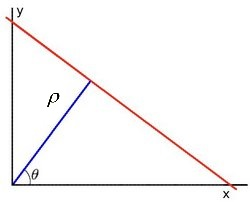
\includegraphics[scale=1]{img/hough-line.jpg}
    \caption{Transformata Hougha w przestrzeni kartezjańskiej}
  \end{center}
  
  \label{rys:maglev}
\end{figure}

Transformata pozwala wykryć linie proste korzystając z faktu, że punkt w przestrzeni $(x,y)$ odpowiada sinusoidzie w przestrzeni Hougha. Z kolei proste są transformowane w punkt. Z tego powodu stosując transformatę Hougha dla linii prostych w przestrzeni $(\rho, \theta)$ zaobserwujemy rodzinę sinusoid, które przecinają się we wspólnym punkcie. To przecięcie stanowi maksimum w obrazie wynikowym.



%\begin{equation} \label{maglev_rown}
%  \begin{cases}
%    \dot{x}_1 & = x_2 \\
%    \dot{x}_2 & = -e^{-x_1} \cdot x_3^2 + 1 \\
%    \dot{x}_3 & = -cx_3 + u
%    \end{cases}
%\end{equation}
%

%Współczynniki przeskalowania zebrano w tabeli.
%
%\begin{table}[!htb]
%  \centering
%  \begin{tabular}{|c|l|l|}
%  \hline
%  Współczynnik & Wartość \\
%  \hline
%  $\alpha$ & $0,00773746 m$ \\
%  \hline
%  $\beta$ & $0,275507681 m/s$ \\
%  \hline
%  $\gamma$ & $0,28890446065998 A$ \\
%  \hline
%  $\xi$ & $0,2808437120924$ \\
%  \hline
%  $\eta$ & $10,28701901522286 A/s$ \\
%  \hline
%  \end{tabular}
%  \caption{Parametry przeskalowania modelu}
%  \label{tab:idf}
%\end{table}


